% !TEX root = ../master-thesis.tex




% \textbf{Introduction and motivation.}
Manipulating the internal spin state of ultracold atoms is an essential element in quantum simulation experiments, particularly for us in context of deterministic state preparation and spin-resolved imaging.
Two widely employed methods for achieving controlled spin transitions in ultracold atomic systems are the Landau-Zener transition and coherent resonant $\pi$-pulse. The Landau-Zener approach involves adiabatically sweeping either the frequency of a driving field or the magnitude of a magnetic field across a spin-resonance. It has been widely applied due to its inherent robustness against small deviations in experimental parameters such as magnetic field fluctuations and frequency drifts. In contrast, the $\pi$-pulse method achieves spin flips by applying a resonant electromagnetic field pulse of precise duration, determined by the corresponding Rabi frequency. Although $\pi$-pulses offer considerably faster spin-flip operations, their fidelity is strongly sensitive to precise calibration of pulse duration, intensity, and frequency detuning, making them more susceptible to experimental noise and parameter instabilities.

Within the context of the current experiment, spin manipulation techniques serve two primary functions. Firstly, flipping atomic spins to stretched states enhances the efficiency of spin-resolved fluorescence imaging. Secondly, selective spin flips are integral to preparation protocols such as spin-selective spilling, allowing controlled removal of atoms in specific spin states. While the Landau-Zener method provided a practical starting point during initial setup stages (mainly due to its robustness against parameter variations) the progression toward faster experimental cycles motivated a transition towards using resonant $\pi$-pulses.

In the following paragraphs, the theoretical foundations of both Landau-Zener and $\pi$-pulse spin manipulation methods are described in detail. A comparative analysis then outlines their respective advantages and limitations in the presence of parameter noise, ultimately justifying the preferred choice adopted in this work.

\textbf{Landau-Zener transition.}
The Landau-Zener (LZ) transition \cite{landau_zur_1932,zener_non-adiabatic_1997} describes the non-adiabatic transition between two quantum states when the energy separation between these states is varied linearly in time. The Hamiltonian governing the dynamics of a two-level system undergoing such a process is expressed as:
\begin{equation}
H_{\text{LZ}}(t) = \frac{\hbar}{2}
\begin{pmatrix}
\Delta(t) & \Omega \\
\Omega & -\Delta(t)
\end{pmatrix},
\label{eq:LZ_Hamiltonian}
\end{equation}
where $\Delta(t)$ represents the instantaneous detuning between the system resonance and the external driving field, and $\Omega$ denotes the coupling strength (Rabi frequency) between the two states. Typically, the detuning is varied linearly as $\Delta(t) = \alpha t$, with $\alpha$ defined as the rate of change of detuning.

The transition probability $P_{\text{LZ}}$, derived analytically under the assumption of a linear sweep and constant coupling, is given by the Landau-Zener formula:
\begin{equation}
P_{\text{LZ}} = 1 - \exp\left(-\frac{\pi \Omega^2}{2\alpha}\right).
\label{eq:LZ_probability}
\end{equation}
This probability explicitly depends on the ratio of the squared coupling strength $\Omega^2$ to the detuning sweep rate $\alpha$. For slow sweeps ($\alpha \ll \Omega^2$), the system achieves near-complete transitions ($P_{\text{LZ}}\rightarrow1$), whereas faster sweeps reduce the fidelity (see Fig.~\ref{fig:spin-flip}b).

An important experimental advantage of the Landau-Zener method is its robustness against fluctuations in experimental parameters, such as variations in the magnetic field or the driving frequency. Small deviations in magnetic field gradients or frequency drifts typically have minimal impact on transition fidelity due to the exponential character of Eq.~\eqref{eq:LZ_probability}. This robustness is particularly valuable in experiments where shot-to-shot variations in magnetic fields are inevitable. Despite its robustness, the Landau-Zener transition requires relatively long timescales ($t_{\text{LZ}} \gg 1/\Omega$) to achieve high transition fidelities, which can slow down experimental cycles and increase exposure to decoherence processes.

\textbf{Rabi $\pi$-pulse.}
An alternative technique for coherent spin manipulation is the resonant Rabi oscillation method, commonly known as the $\pi$-pulse approach. This method exploits coherent driving of the transition between two spin states at constant resonance, enabling deterministic and rapid population transfer.

The dynamics under resonant excitation are described by the Hamiltonian in Eq.~\eqref{eq:LZ_Hamiltonian} with a constant detuning $\Delta=\text{const}$. By applying a resonant driving field ($\Delta=0$) for the duration $t_\pi = \pi/\Omega$, the system achieves complete inversion of the spin populations, thus realizing an ideal spin-flip operation between states $\ket{1}$ and $\ket{2}$.

The primary advantage of the $\pi$-pulse technique is its speed: the required pulse duration is significantly shorter than that for Landau-Zener sweeps ($t_\pi \ll t_{\text{LZ}}$), as evidenced by rapid Rabi oscillations in Fig.~\ref{fig:spin-flip}c. However, the fidelity of $\pi$-pulse transitions is highly sensitive to deviations from the exact resonance condition ($\delta \neq 0$), as well as inaccuracies in pulse duration and field amplitude. This sensitivity is captured analytically by the generalized Rabi oscillation formula:
\begin{equation}
P_{\pi} = \frac{\Omega^2}{\Omega^2+\delta^2}\sin^2\left(\frac{\sqrt{\Omega^2+\delta^2}}{2}t_{\pi}\right).
\label{eq:pi_fidelity}
\end{equation}

Shot-to-shot fluctuations, especially those in the magnetic field, directly translate into variations in resonance conditions and consequently introduce systematic and random errors in spin-flip fidelity. As a result, consistently high fidelity using $\pi$-pulses necessitates stringent experimental stabilization of magnetic fields, pulse timing, and amplitude calibration.


\begin{figure}
    \centering
    \addletter{105}{a}
    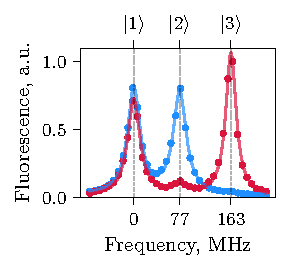
\includegraphics{fig-py/spin-flip-1.pdf}  \phantom{4}
    \addletter{105}{b}
    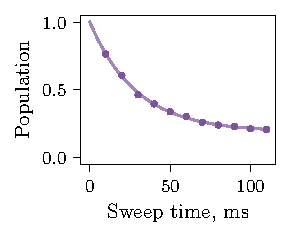
\includegraphics{fig-py/spin-flip-2.pdf}  \phantom{4}
    \addletter{105}{c}
    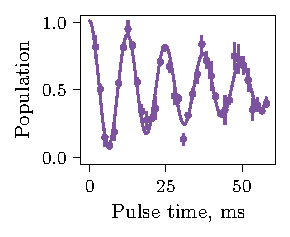
\includegraphics{fig-py/spin-flip-3.pdf}  \phantom{4}
    \caption{
        \textbf{Characterization of spin manipulation protocols.}
        (a) Fluorescence signal measured in the ODT before (blue) and after (red) applying a Landau-Zener sweep between states $\ket{2}$ and $\ket{3}$, showing population transfer to the target state. 
        (b) Final population in $\ket{2}$ as a function of sweep duration, consistent with the Landau-Zener model. 
        (c) Rabi oscillations observed when applying resonant RF $\pi$-pulse between states $\ket{2}$ and $\ket{3}$, demonstrating coherent control of the spin transition.
    }
    \label{fig:spin-flip}
\end{figure}


% \textbf{In this experiment.}
In the present experiment, spin-state populations are routinely measured by scanning the laser frequency while simultaneously recording the fluorescence signal of atoms either confined in the ODT or directly in optical tweezers. Figure~\ref{fig:spin-flip}a demonstrates a typical example, showing clear fluorescence peaks corresponding to distinct spin states. Such spectral scans provide a reliable quantitative method for assessing the efficiency of spin-state transitions.
% 
Initially, spin manipulation in this experiment relied primarily on Landau-Zener sweeps. 
% Operating at moderate coupling strengths ($\Omega \sim 1~\text{kHz}$), transition fidelities around \red{95\%} were achieved. 
Subsequent technical improvements in the RF and MW antenna designs allowed increasing the effective coupling strength up to approximately 10~kHz. Employing $\pi$-pulses at this higher coupling strength consistently yielded fidelities of \red{99\%}.

In conclusion, while Landau-Zener sweeps provided a robust and convenient method for spin-state manipulation during initial setup phases, the improvements in RF/MW coupling strengths ultimately favored the adoption of faster and more efficient $\pi$-pulse protocols.